% Chapter 1
\section*{\centering Preface}
This chapter discusses the characterisation techniques that were implemented post-mortem, to fully analyse how a battery works. Electrochemical processes such as cyclic voltammetry and galvanostatic charge/ discharge curves have been discussed in detail.   

\pagebreak

\chapter{Techniques for characterisation} % Main chapter title

\label{chap2} % For referencing the chapter elsewhere, use \ref{Chapter1} 

Performance of a battery cannot be assessed without galvanostatic charge and discharge cycles and cyclic voltammetry (CV). CV scans help in determining the voltage range of a cell and the upper cut-off of the voltage range is determined by the stability of the electrolyte. A charge/discharge cycle (CDC) on the other hand helps in evaluating a cell's specific capacity and nominal (discharge) voltage. Long term CDCs are necessary to verify a cell's stability and observe whether it can be put to commercial use or not. 
During continuous charge and discharge, a cathode material undergoes many changes. For example, distance between two layers may increase due to intercalation of ions. Or, the oxidation states of a metal may change when it oxidises or reduces itself during cycles. Analytical tools are needed to study the following. 

\begin{itemize}
    \item Changes in the crystal lattice of a material can be studied from its X-ray diffraction patterns (XRD)
    \item Changes in the oxidation state of an element can be observed from its X-ray photoelectron spectra (XPS)
    \item Changes in the vibrational modes of a molecule can be observed from its Raman spectra 
\end{itemize}

\section{Galvanostatic charge/discharge cycles}
Galvanostatic charge/discharge is a method to evaluate the amount of charge capable of being stored in a cell. The technique measures voltage at a fixed current rate. Since the charging and discharging current is kept constant, the voltage adjusts to deliver that set current. The graph below shows a typical charge/discharge curve for an AIB when charged and discharged at a constant current rate of 50 mA g$^{-1}$. Each cell chemistry has its own characteristic nominal voltage and discharge curve. Lithium batteries have a fairly flat discharge curve while others such as lead-acid have a pronounced slope. A sloping discharge curve means that the power falls gradually throughout the discharge. A flatter curve means less voltage variations and the voltage remains constant throughout the discharge cycle which is desirable for many applications. The battery analyser plots the voltage against time and helps in determining the nominal voltage of the cell. The charge/ discharge cycles help in determining the specific capacity and cycling stability of a cell. As mentioned in Chapter \ref{chap1}, the effective capacity of the cell is reduced if the cell is discharged at very high current rates (or conversely increased with low discharge rates). Discharging the cell at a high current rate decreases the cell voltage quickly so that only a part of capacity can be used. The total quantity of electricity per mass available from a fully charged cell can be calculated, from the charge transferred during discharge in terms of mAh g$^{-1}$. Specific discharge capacity is frequently measured at different discharging rates to establish rate capability of a cell \cite{pyun_electrochemistry_2012-2}. The voltage profile obtained can be used to identify multi-step redox reactions shown in Figure \ref{Figures/chap2fig:ChrononCDC}. A few other terms associated with the charge/ discharge cycle are:
\begin{itemize}
\item Self-discharge: Self discharge rate is a measure of how quickly a cell will lose its energy while sitting on the shelf due to unwanted chemical reactions within the cell. The rate depends on the cell chemistry and the temperature. Self-discharge, which occurs in all batteries, determines the \enquote{shelf life} of a battery.
\item Trickle charging or slow charging: \enquote{Slow charge} is defined as a charging current that can be safely applied to a battery indefinitely without any kind of charge termination method. LIBs do not tolerate trickle charging after they are fully charged. Further charging (even a small amount of current) a fully charged LIB damages it. For this reason, lithium cells are charged using constant- voltage (C-V) chargers, and not constant- current (C-C) chargers.

\end{itemize}

\begin{figure}[th!]
\centering
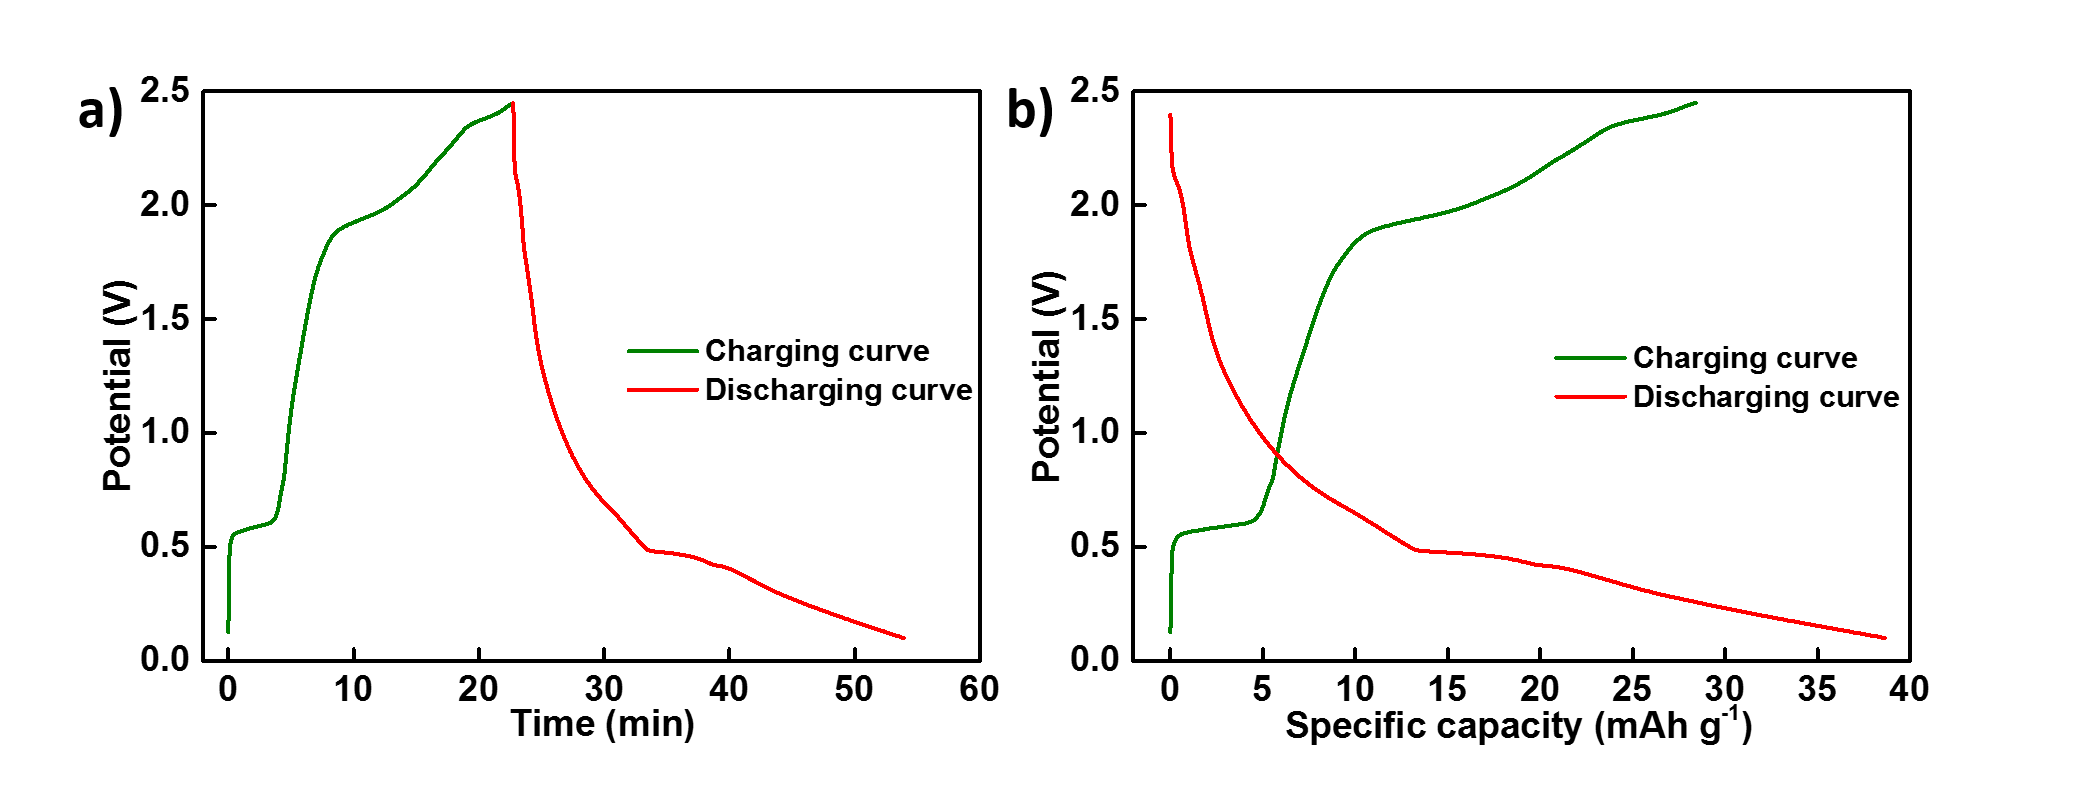
\includegraphics[width=\textwidth]{Figures/chap2fig/ChrononCDC}
\caption{a) Chronopotentiogram: a graph of battery potential versus time, at constant current. b) A galvanostatic charge/discharge curve showing the voltage plateaus at which reactions occur and the charging/discharging capacity.}
\label{Figures/chap2fig:ChrononCDC}
\end{figure}

\section{Cyclic voltammetry}
Cyclic voltammetry (CV) is a technique which measures the current that develops in an electrochemical cell during oxidation and reduction of an analyte (M). It is performed by cycling the potential of a working electrode, and measuring the resulting current. In Figure \ref{Figures/chap2fig:CV}, the voltage was scanned from a lower voltage to a higher voltage (positive scan). S1 is called the upper limit or the upper cut-off, where the voltage is sufficient enough to cause an oxidation or reduction. Once the voltage reaches S1, the direction of the scan is reversed. Potential is then swept negatively (higher potential to lower potential) until it reaches S2 (another switch potential). In an ideal situation, during forward sweep, M is depleted from the solution as it gets oxidised to \ce{M+}. Further oxidation after scanning higher potentials, leads to growth of a diffusion layer (solution containing M/\ce{M+} ions) at the electrode surface throughout the scan. The layer continues to expand until a certain point, recording maximum current density. However, since diffusion layer continues to grow at this stage, flux of M from the bulk solution to electrode surface decreases. Therefore, current starts to decrease and we get an oxidation peak. A reverse scan converts \ce{M+} back to M (reduction) via similar pathway- formation of a diffusion layer containing M and eventually a reduction peak is recorded. If the reduction process is chemically and electrochemically reversible, a peak-to-peak separation of 59 mV is observed. When there is a high barrier to electrochemical irreversibility, electron transfer reactions are sluggish and more positive/negative potentials are required to observe oxidation/reduction reactions respectively. 

\begin{figure}[tbh!]
\centering
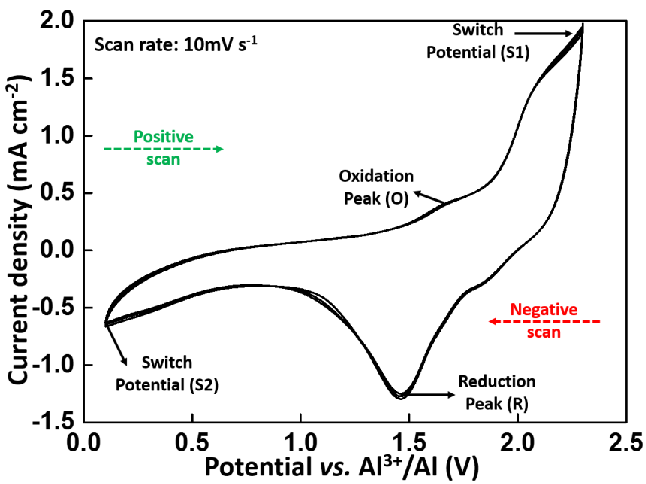
\includegraphics[width=0.8\textwidth]{Figures/chap2fig/CV.pdf}
\caption{Cyclic voltammogram of an AIB at a scan rate of 10 mV s$^{-1}$ using a two-electrode cell with aluminium foil acting as both the counter and reference electrode.}
\label{Figures/chap2fig:CV}
\end{figure}

\begin{figure}[tbh!]
\centering
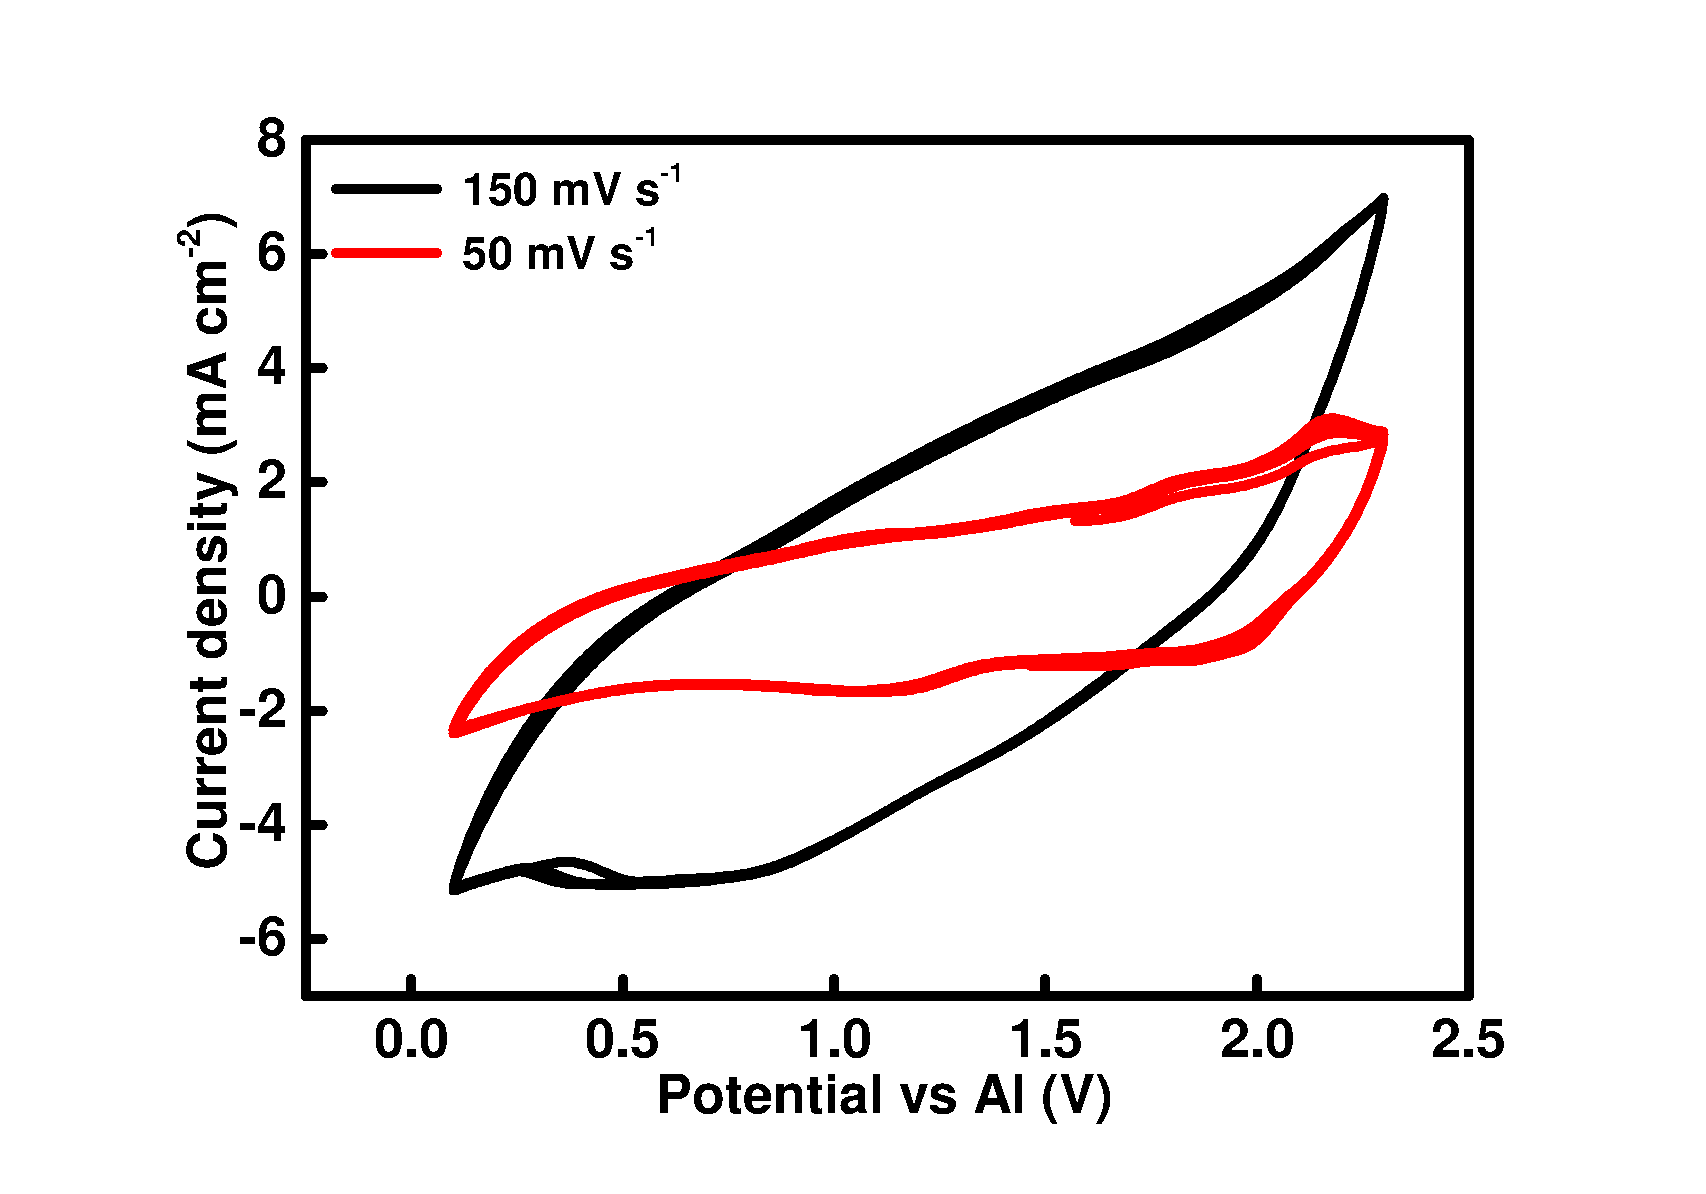
\includegraphics[width=0.8\textwidth]{Figures/chap2fig/scanrate.pdf}
\caption{Cyclic voltammogram of an aluminium-ion battery using human hair as the cathode at different scan rates.}
\label{Figures/chap2fig:scanrate}
\end{figure}

Scan rates play a very important role too. If a CV is run on a slower scan rate, e.g. 0.05 mV s$^{-1}$, diffusion layer grows farther from the electrode, which reduces the flux, consequently decreasing the current value. At a faster scan rate (1 V s$^{-1}$), the size of the diffusion layer decreases and higher currents are recorded as shown in Figure \ref{Figures/chap2fig:scanrate}. Cyclic voltammetry is a helpful tool in understanding the presence of a surface reaction. The presence of oxidation and reduction peaks, distance between two peaks, and the overlapping of peaks after each scan gives a lot of information about the reversibility during cell cycles. It can be used for both single-electron and multi-electron processes.  
After a cell has been assembled, the electrochemical processes such as galvanostatic CDCs or CVs are measured. However, to investigate the impact of continuous cycling on the cathode material, the electrode has to be separated from the main cell and analysed. 
\section*{Sample preparation}
The cell was disassembled inside a glove box to prevent the cathode from any contact with air or moisture. The cathode was taken out and washed with dry ethanol to get rid of any remaining electrolyte on its surface. It was found that scrapping off the active material from the current collector did not yield enough sample for analysis, since some of it got washed away in the process. Thus, cathode coated on Mo foil was treated as a sample for X-ray diffraction, Raman and X-ray photoelectron spectroscopic analyses.

\section{X-ray diffraction studies}
Diffraction of x-rays by crystal planes allows us to derive lattice spacings by using Bragg's law. 

 \begin{equation} \label{eq2-1}
     2d\sin\theta \text= n{\lambda}
 \end{equation}
 where d = spacing between diffracting planes,\\
$\theta$ = incident angle,\\ 
n = any positive integer, and \\
$\lambda$ = wavelength of the incident beam.\\
X-rays produce the diffraction pattern because their wavelength $\lambda$ is typically the same order of magnitude (1-10 \AA) as the d-spacing between the crystal planes. According to equation \ref{eq2-1} any decrease in 2$\theta$ suggests an increase in the d-spacing. A pure crystalline sample such as \ce{MoS2} (Figure \ref{Figures/chap2fig:XRD} a) yields sharp peaks in a XRD pattern since it has a long-range ordered structure. Random orientation of the powdered material is attained after scanning the sample through a range of 2$\theta$ angles. Conversion of the diffraction peaks to d-spacings allows identification of the sample because each sample has a unique set of d-spacings. Typically, d-spacings of the sample are compared with standard reference patterns (International Centre for Diffraction Data, ICDD). For determination of unit cell parameters, each reflection implies a specific lattice plane indicated by Miller indices \textit{hkl} (labelled in red  for \ce{MoS2} crystal lattice). Figure \ref{Figures/chap2fig:XRD} b displays the diffraction pattern of activated carbon obtained from human hair. Since the structure of activated carbon is much less ordered, the patterns shows line broadening of the major diffraction bands, which exist at $\sim$ 25$^{\circ}$  and $\sim$ 44$^{\circ}$.
X-ray diffraction studies is a useful tool and helps in revealing the structural changes that go inside a cell during intercalation of ions. Rani \textit{et al.} used fluorinated graphite as a cathode for AIBs. The d-spacing values of the discharged graphite cathode were higher than natural graphite. This indicated that intercalation of \ce{Al^3+} ions in the graphene sheets increase the d-spacing of the crystal lattice\cite{rani_fluorinated_2013}.
%X-ray diffraction shows line broadening of only the principal graphite diffraction bands. This broadening is usually interpreted in terms of dimensions of a hypothetical crystallite. Although the crystallite concept has been used when comparing structures in carbons, it has to be stressed that the crystallite does not exist as such within these structures. The disorganized carbon are present in cross-linkage structures [15] forming non-crystallite structures to form microstructures! 
Panalytical X-Ray diffractometer was used to record the XRD patterns using Cu-K$\alpha$ radiation at an operating voltage of 45 kV and a 40 mA current. The patterns were run with copper radiation ($\lambda$ =1.5405\AA) at a scanning speed of 2$^{\circ}$ in 20 minutes. 

\begin{figure}[tbh!]
\centering
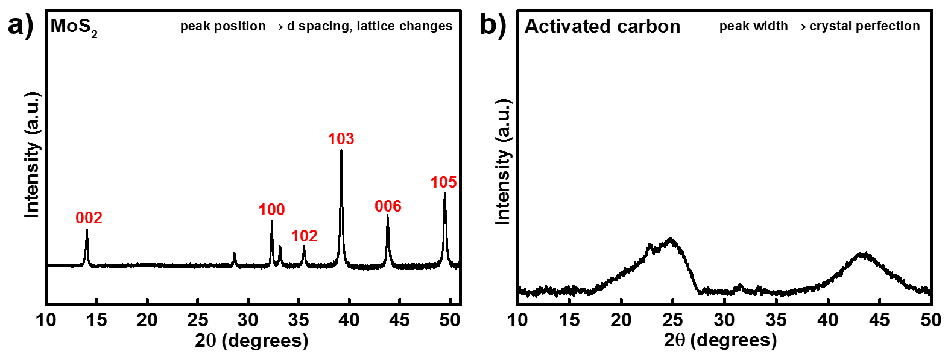
\includegraphics[width=\textwidth]{Figures/chap2fig/XRD.pdf}
\caption{X-ray diffraction pattern of a) bulk molybdenum disulfide (ICDD: 04-001-9285), and b) activated carbon.}
\label{Figures/chap2fig:XRD}
\end{figure}

\section{Raman spectroscopy}
Raman spectroscopy is a technique, which is used to study vibrational modes of a molecule. A source of monochromatic light, usually from a laser, interacts with molecular vibrations in the system, resulting in the energy of the laser photons being shifted up (blue shift) or down (red shift). The shift in energy gives information about any changes taking place in the vibrational modes of a material. 
%This technique uses the inelastic scattering of photons, also known as Raman scattering. 
\begin{figure}[tbh!]
\centering
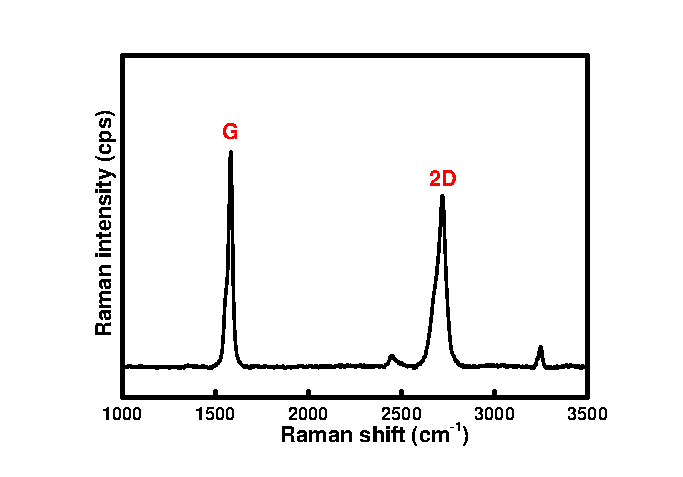
\includegraphics[width=\textwidth]{Figures/chap2fig/Raman.pdf}
\caption{Raman spectra of graphite with prominent G and D bands labelled.}
\label{Figures/chap2fig:Raman}
\end{figure}

Graphite is composed of sp$^2$ bonded carbon atoms in planar sheets. The bond energy of the sp$^2$ bonds displays its vibrational frequency at 1582 cm$^{-1}$. The presence of additional bands in the graphite spectrum indicate that there are some carbon bonds at different bond energies. The D band indicates presence of some disorder in the structure (Figure \ref{Figures/chap2fig:Raman}). The G band is an outcome of in-plane vibrations, whereas the D peak is due to out of plane vibrations attributed to the presence of structural defects. If the D band is more intense, it means that the sp$^2$ bonds are broken which in turn means that there are more sp$^3$ bonds present. The ratio of intensity of D/G peaks is a measure of the defects present. Both D and G peaks are the result of vibrations of sp$^2$ bonded carbon atoms.  
Raman spectroscopy is a helpful technique in detecting the mechanism of an intercalation-based battery. It is most sensitive to highly symmetric covalent bonds with little or no natural dipole moment. The C-C bonds fit this criterion perfectly and as a result Raman spectroscopy is highly sensitive to these materials and provides a wealth of information about their structure. Wang \textit{et al.} used Raman spectroscopy to show two different intercalation processes involving chloroaluminate anions in a graphite cathode in an AIB, shown in Figure \ref{Figures/chap2fig:Raman2}. The data displayed two different intercalation processes at two different charging plateaus. The first plateau in the charging curve showed G band splitting and the higher voltage plateau exhibited a single, dominant blue-shifted peak. During discharge, the opposite trends were observed when chloroaluminate anions were deintercalated. The original graphite spectrum was recovered when the cell was fully discharged\cite{wang_advanced_2017}. 

\begin{figure}[tbh!]
\centering
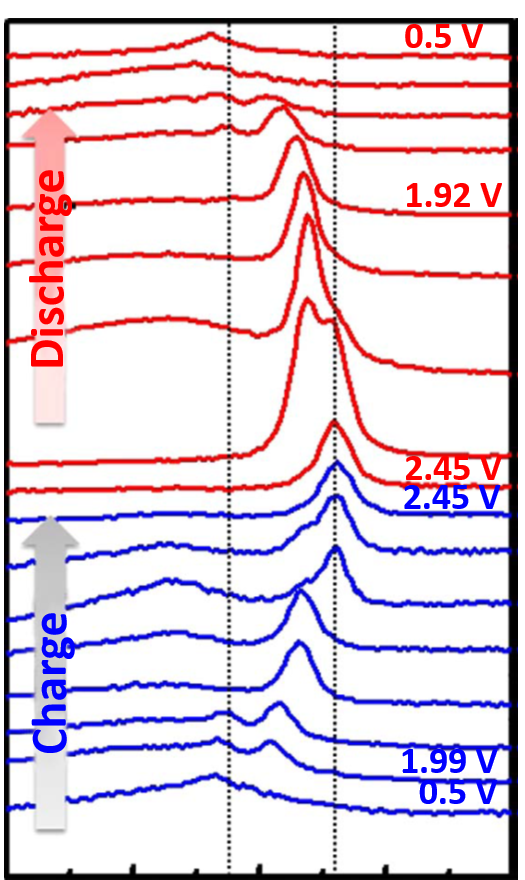
\includegraphics[width=0.5\textwidth]{Figures/chap2fig/Raman2}
\caption{\textit{In-situ} Raman spectra recorded for the natural graphite cathode through a charge–discharge cycle showing chloroaluminate anion intercalation/ de-intercalation into graphite \cite{wang_advanced_2017}. Permissions not required.}
\label{Figures/chap2fig:Raman2}
\end{figure}

\section{X-ray photoelectron spectroscopy}
 X-ray photoelectron spectroscopy is used to measure elemental composition and oxidation states of various elements. It is a surface-based technique that quantitatively analyses a sample. By irradiating a sample with a beam of X-rays, kinetic energy and number of electrons escaping from the top 10 nm of the sample are measured. 
%The instrument requires high vacuum (10$^{-8}$ millibar) conditions to count these electrons. The electron emission after irradiation is also called a 'photoelectron effect'. These electrons are separated according to their energies and counted. ,
A normal XPS spectrum plots the number of electrons detected versus the binding energy of the electrons. XPS helps in characterising elements species and valence changes of original sample and sample during electrochemical reactions. It helps in studying the redox processes that take place inside a cell. Understanding curve-fitting of an XPS spectra is an important aspect since it suggests the number of chemical states present in a sample. Figure \ref{Figures/chap2fig:XPS} displays a detailed narrow spectrum scan of molybdenum. It can been seen that the binding energies of Mo 3d include a pair of peaks at 232.3 and 229.1 eV, which are attributed to Mo 3d$_{3/2}$ and Mo 3d$_{5/2}$ in \ce{MoS2}, respectively\cite{grim_x-ray_1975}. Furthermore, it is essential to apply constraints to restrict peak widths and relative intensities of the peaks in a spectra. All the peaks in this thesis were fitted using a Shirley background and any observed peak was deconvoluted using Gaussian and Lorentzian function. \\
Li \textit{et al.} studied the XPS spectra of \ce{MoS2} microspheres to probe the valence changes and the Al$^{3+}$ storage mechanism during the charging/ discharging process at various charge and discharge states of the cathode \cite{li_rechargeable_2018}.

\begin{figure}[tbh!]
\centering
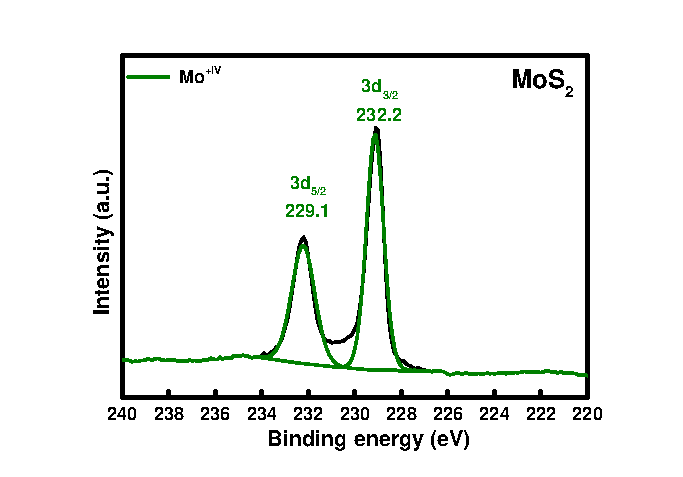
\includegraphics[width=\textwidth]{Figures/chap2fig/XPS.pdf}
\caption{X-ray photoelectron spectra of molybdenum disulfide. Molybdenum 3d orbitals appear as a doublet at 229 and 232 eV. The area ratio for the two peaks (3d$_{3/2}$ : 3d$_{5/2}$) was 2:3 (corresponding to two electrons in the 3d$_{3/2}$ level and 4 electrons in the 3d$_{5/2}$ level).}
\label{Figures/chap2fig:XPS}
\end{figure}




